\documentclass[]{minimal}
\usepackage{tikz}
\usetikzlibrary{positioning}
\usetikzlibrary{arrows}

\begin{document}

\pagestyle{empty}

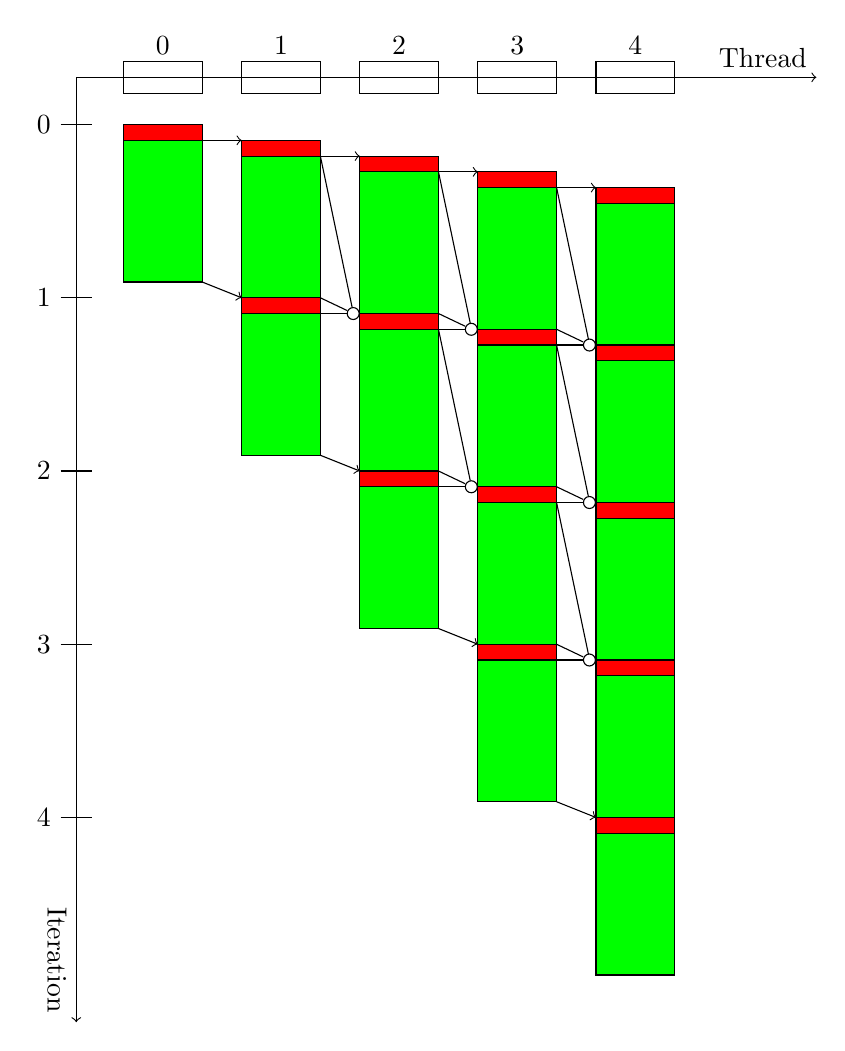
\begin{tikzpicture}[scale=2]
    \newcommand\Threads{4}
    \newcommand\Threadsmm{3}

    % Y-Axis
    \draw[->] (-.3,.3) -- (-.3,-1*\Threads-1.7) node[pos=1,below left, sloped] {Iteration};
    \foreach \x in {0,...,\Threads} {
        \draw (-.4, -1.1*\x) -- (-.2, -1.1*\x) node [pos=0, left] {\x};
    }

    % X-Axis
    \draw[->] (-.3,.3) -- (.75*\Threads+1.4,.3) node[pos=1,above left] {Thread};
    \foreach \x in {0,...,\Threads} {
        \draw(.75*\x, .2) rectangle (.5+0.75*\x, .4);
        \node at (0.75*\x+.25,.5) {\x};
        }


    % Computatations
    \foreach \y in {0,...,\Threads} {
        \foreach \x in {\y,...,\Threads} {
            \draw[fill=red] (.75*\x,-\y-.1-.1*\x) rectangle (.5+0.75*\x, -\y-.1*\x);
            \draw[fill=green] (.75*\x,-\y-1-.1*\x) rectangle (.5+0.75*\x, -\y-.1-.1*\x);
        }
    }

    % Communication
    % init
    \foreach \x in {0,...,\Threadsmm} {
        \draw[->] (.5+0.75*\x,-.1*\x-.1) -- (.75+0.75*\x,-.1*\x-.1);
    }
    % first of every iteration
    \foreach \x in {0,...,\Threadsmm} {
        \draw[->] (.5+0.75*\x,-1.1*\x-1) -- (.75+0.75*\x,-1.1*\x-1.1);
    }
    % merges
    \foreach \y in {1,...,\Threadsmm} {
        \foreach \x in {\y,...,\Threadsmm} {
        % previous coarse
        \draw[shorten >=0.08cm] (.5+0.75*\x,-\y-.1*\x+.9) -- (.71+0.75*\x,-\y-.1-.1*\x);
        % fine
        \draw[ shorten >=0.09cm] (.5+0.75*\x,-\y-.1*\x) -- (.71+0.75*\x,-\y-.1-.1*\x);
        % coarse
        \draw[-o, shorten >=0.0cm] (.5+0.75*\x,-\y-.1*\x-.1) -- (.75+0.75*\x,-\y-.1-.1*\x);
        }
    }



\end{tikzpicture}


\end{document}